%! TeX root: ../informe.tex
\section{Resultados y discusión}
\label{sec:results}

\setlength{\emergencystretch}{6em}
\sloppy
\setlength{\tabcolsep}{4pt}

La tabla~\ref{tab:catalogo-experimentos} resume los barridos ejecutados. Cada
uno varía un único eje alrededor de una configuración base común para que las
comparaciones sean justas; las subsecciones siguientes se refieren a cada barrido
por su identificador. A lo largo de la discusión las métricas intrínsecas
(silueta~$\uparrow$, CH~$\uparrow$, DB~$\downarrow$;
\ref{subsubsec:metricas}) se leen siempre de forma conjunta con el número de
clústeres, la fracción de ruido y el coeficiente de variación de los tamaños:
leídas de forma aislada, la silueta y el CH premian configuraciones degeneradas
(particiones binarias triviales o pocos clústeres grandes), por lo que el juicio
se emite sobre el criterio conjunto.

{\footnotesize
\begin{longtable}{|p{0.6cm}|p{3.9cm}|p{3.6cm}|p{4.7cm}|} \hline
  \textbf{Id} & \textbf{Elementos variados} & \textbf{Fijo} & \textbf{$N$ / repeticiones} \\ \hline
  \endhead
  E1 & Extractor & UMAP-10, HDBSCAN \texttt{mcs}=5, identidad, SQLite & $N\in\{250, 1000, 6416\}$, $K{=}3$ \\ \hline
  E2 & Reducción & Extractor base, HDBSCAN \texttt{mcs}=5 & $N\in\{250, 1000, 6416\}$, $K{=}3$ \\ \hline
  E3 & Agrupamiento & Extractor base, UMAP-10 & $N\in\{250, 1000, 6416\}$, $K{=}3$ \\ \hline
  E4 & HDBSCAN \texttt{min\_cluster\_size} & Extractor base, UMAP-10 & $N\in\{250, 1000, 6416\}$, $K{=}3$ \\ \hline
  E5 & Segmentador & \textit{Pipeline} base & $N\in\{250, 1000, 6416\}$, $K{=}3$ \\ \hline
  E6 & Almacenamiento & \textit{Pipeline} base, búsqueda activa & $N\in\{500, 1000, 2500, 6416\}$, $K{=}5$ \\ \hline
  E7 & $N$ $\times$ agrupamiento & Extractor base, UMAP-10, SQLite & $N\in\{250, 500, 1000, 2000,$ $3500, 6416\}$, $K{=}5$ \\ \hline
  E8a & Extractor $\times$ red.\ $\times$ agrup.\ (estilo) & SQLite, identidad, sin límite & 294 recortes, 4 clases, $K{=}3$ \\ \hline
  E8b & Extractor $\times$ red.\ $\times$ agrup.\ (autoría) & SQLite, identidad, sin límite & 185 recortes, 87 autores, $K{=}3$ \\ \hline
  E9 & Parámetros HNSW & \textit{Pipeline} base, PostgreSQL & $N{=}6416$, $K{=}5$ \\ \hline
  \caption[Catálogo de barridos experimentales]{Catálogo de barridos experimentales.}
  \label{tab:catalogo-experimentos}
\end{longtable}
}

\subsection{Calibración del \textit{pipeline}}
\label{subsec:res-calibracion}
Esta sección fija el \textit{pipeline} base sobre el que se asientan los estudios
de coste y calidad supervisada. La elección de reducción, agrupamiento y
segmentador queda decidida por E2--E5; la del extractor se basa en la calidad
supervisada (E8a), discutida en \ref{subsec:res-supervisada}.

\subsubsection{Extractor de características.}
Se prueban doce extractores: cuatro CNN preentrenadas en ImageNet,
\texttt{dinov2\_vits14}, \texttt{clip\_vit\_b32}, dos \textit{backbones} YOLO y
la matriz $2\times2$ de cabezas \textit{fine-tuned} (autor y estilo $\times$
DINOv2 y MobileNetV3). La tabla~\ref{tab:e1-quality-6416} recoge la calidad
intrínseca a $N=6416$. El resultado más llamativo es la inversión entre silueta
y CH en ambas cabezas estilísticas: la silueta cae respecto a su
\textit{backbone} (DINOv2 $0.185\to0.155$; MobileNetV3 $0.260\to0.164$) mientras
el CH sube (DINOv2 $19.2\to27.9$; MobileNetV3 $13.1\to19.7$). El
\textit{contrastive loss} optimiza la compactación y separación de clústeres
(CH), no la cohesión local de cada punto (silueta), y el cambio de dominio
(las cabezas se entrenaron con recortes, aquí se evalúan imágenes completas)
agrava la caída. Las CNN de ImageNet lideran la silueta con ruido bajo y
clústeres balanceados, pero probablemente agrupan por apariencia genérica
(textura, color, composición) sin codificar información relevante de grafiti;
YOLO pierde en casi todos los ejes, confirmando que sus características de
detección no transfieren a un agrupamiento por apariencia.

{\footnotesize
\begin{longtable}{|p{5.0cm}|p{0.9cm}|p{0.9cm}|p{0.9cm}|p{0.9cm}|p{0.9cm}|p{0.9cm}|} \hline
  \textbf{Extractor} & \textbf{cls} & \textbf{ruido} & \textbf{sil} & \textbf{CH} & \textbf{DB} & \textbf{csCV} \\ \hline
  \endhead
  \texttt{mobilenet\_v3}                  & 820 & \textbf{0.078} & \textbf{0.260} & 13.1 & 1.48 & \textbf{0.52} \\ \hline
  \texttt{resnet50}                       & 794 & 0.086 & 0.257 & 15.6 & \textbf{1.46} & 0.71 \\ \hline
  \texttt{vgg16}                          & 773 & 0.095 & 0.228 & 13.4 & 1.55 & 0.54 \\ \hline
  \texttt{mob.\_graffiti\_author\_head}   & 779 & 0.124 & 0.227 & 13.4 & 1.53 & 0.53 \\ \hline
  \texttt{inception\_v3}                  & 724 & 0.118 & 0.213 & 11.5 & 1.61 & 0.64 \\ \hline
  \texttt{dinov2\_graffiti\_author\_head} & 631 & 0.143 & 0.187 & 17.9 & 1.59 & 0.81 \\ \hline
  \texttt{dinov2\_vits14}                 & 632 & 0.123 & 0.185 & 19.2 & 1.58 & 0.92 \\ \hline
  \texttt{clip\_vit\_b32}                 & 734 & 0.150 & 0.170 & 11.9 & 1.66 & 0.74 \\ \hline
  \texttt{mob.\_graffiti\_style\_head}    & 629 & 0.214 & 0.164 & 19.7 & 1.74 & 0.58 \\ \hline
  \texttt{dinov2\_graffiti\_style\_head}  & 562 & 0.202 & 0.155 & 27.9 & 1.70 & 0.74 \\ \hline
  \texttt{yolom}                          & 480 & 0.253 & 0.131 & 32.2 & 1.75 & 0.74 \\ \hline
  \texttt{yolon}                          & 348 & 0.341 & 0.085 & \textbf{51.2} & 1.91 & 0.81 \\ \hline
  \caption[E1, calidad intrínseca a $N=6416$]{E1, calidad intrínseca a $N=6416$. El extractor base
  (\texttt{dinov2\_graffiti\_style\_head}) presenta un CH solo superado por los
  \textit{backbones} YOLO, pese a una silueta inferior a la de su
  \textit{backbone}. \glosacalidad}
  \label{tab:e1-quality-6416}
\end{longtable}
}

En coste (tabla~\ref{tab:e1-cost-6416}), \texttt{mobilenet\_v3} es el más barato
en velocidad y VRAM (7.93~ips, 32~MB) y la cabeza añade un sobrecoste pequeño
($\sim$8\%); los \textit{backbones} YOLO son los más caros en tiempo y RSS, y
VGG16/CLIP los más exigentes en VRAM.

{\footnotesize
\begin{longtable}{|p{5.0cm}|p{1.6cm}|p{0.9cm}|p{1.3cm}|p{1.3cm}|} \hline
  \textbf{Extractor} & \textbf{ingesta (s)} & \textbf{ips} & \textbf{RSS (MB)} & \textbf{VRAM (MB)} \\ \hline
  \endhead
  \texttt{mobilenet\_v3}                  & \textbf{808.8}  & \textbf{7.93} & 366.0 & \textbf{31.8}  \\ \hline
  \texttt{mob.\_graffiti\_author\_head}   & 879.1  & 7.30 & 406.4 & 34.5  \\ \hline
  \texttt{inception\_v3}                  & 973.7  & 6.59 & 337.2 & 116.1 \\ \hline
  \texttt{vgg16}                          & 980.8  & 6.54 & 315.0 & 551.7 \\ \hline
  \texttt{resnet50}                       & 1080.0 & 5.94 & 336.0 & 117.8 \\ \hline
  \texttt{dinov2\_vits14}                 & 1215.7 & 5.28 & 209.6 & 98.0  \\ \hline
  \texttt{dinov2\_graffiti\_style\_head}  & 1245.0 & 5.15 & 286.2 & 99.7  \\ \hline
  \texttt{clip\_vit\_b32}                 & 1247.0 & 5.15 & \textbf{193.1} & 591.9 \\ \hline
  \texttt{yolon}                          & 1301.0 & 4.93 & 853.8 & 65.4  \\ \hline
  \texttt{yolom}                          & 1407.4 & 4.56 & 824.9 & 192.9 \\ \hline
  \caption[E1, coste de ingesta a $N=6416$.]{E1, coste de ingesta a $N=6416$ (10 de 12 extractores; las dos
  cabezas omitidas caen dentro del rango de la cabeza correspondiente). La cabeza
  añade un sobrecoste despreciable sobre el \textit{backbone}.}
  \label{tab:e1-cost-6416}
\end{longtable}
}

\subsubsection{Reducción de dimensionalidad.}
Sobre los vectores de 128 dimensiones del extractor base, el barrido E2 revela a
UMAP como la única familia que produce simultáneamente un número de clústeres no
trivial, ruido moderado y tamaños balanceados
(tabla~\ref{tab:e2-quality-6416}). La fila \emph{identidad} responde a cuánto
aporta la reducción: agrupando los 128-d crudos, HDBSCAN agrupa solo un núcleo
denso y descarta el 68\% de los puntos como ruido, una segmentación de cobertura
muy baja que las métricas individuales premian engañosamente (silueta $0.307$,
DB $1.16$). PCA-10 colapsa a $k=2$ y PCA-50 explota a $k=238$ con un 70\% de
ruido. Además, la identidad no es gratuita: empuja el coste a la etapa de
agrupamiento (HDBSCAN tarda 6.83~s sobre la identidad frente a 0.34~s sobre
UMAP-10, $\sim$20 veces más), e Isomap-10 es lo más caro del experimento
(23.9~s, 1.25~GB) para una partición igualmente degenerada. UMAP-10 y UMAP-50 son
indistinguibles en calidad, pero UMAP-50 cuesta casi el doble; de ahí la
recomendación específica de UMAP con \texttt{n\_components=10}.

{\footnotesize
\begin{longtable}{|p{2.0cm}|p{1.0cm}|p{1.0cm}|p{1.2cm}|p{1.0cm}|p{1.0cm}|p{1.0cm}|} \hline
  \textbf{Reducción} & \textbf{cls} & \textbf{ruido} & \textbf{sil} & \textbf{CH} & \textbf{DB} & \textbf{csCV} \\ \hline
  \endhead
  identidad   & 301 & 0.684 &  \textbf{0.307} & 37.5 & \textbf{1.16} & \textbf{0.55} \\ \hline
  PCA-10      & 2   & 0.010 &  0.000 &  4.2 & 1.39 & 1.00 \\ \hline
  PCA-50      & 238 & 0.698 &  0.238 & 36.6 & 1.29 & 2.29 \\ \hline
  UMAP-10     & 562 & 0.202 &  0.155 & 27.9 & 1.70 & 0.74 \\ \hline
  UMAP-50     & 558 & \textbf{0.195} &  0.154 & 27.8 & 1.71 & 0.70 \\ \hline
  Isomap-10   & 125 & 0.624 &  0.044 & \textbf{38.4} & 1.80 & 3.40 \\ \hline
  \caption[E2, calidad intrínseca a $N=6416$]{E2, calidad intrínseca a $N=6416$. UMAP es la única reducción que
  produce simultáneamente un número de clústeres no trivial, ruido moderado y
  tamaños balanceados. \glosacalidad}
  \label{tab:e2-quality-6416}
\end{longtable}
}

\subsubsection{Algoritmo de agrupamiento.}
El barrido E3 cubre 14 configuraciones sobre el extractor base y UMAP-10;
la tabla~\ref{tab:e3-summary-6416} extrae la fila representativa de cada familia
y la figura~\ref{fig:e3-pareto} muestra el frente de calidad frente a coste.
Como los algoritmos de densidad se juzgan solo sobre el subconjunto que agrupan
y los particionales sobre el conjunto completo, el criterio conjunto es
imprescindible. Bajo él, HDBSCAN es el único agrupador que combina silueta
competitiva, escalado sensato del número de clústeres con $N$, ruido moderado,
tamaños balanceados y coste despreciable. OPTICS es su único par en calidad
(superándolo ligeramente en silueta), pero queda dominado en coste ($\sim$25
veces más tiempo y $\sim$2500 veces más memoria a $N=6416$). Entre los
particionales, GMM con $k$ por BIC es la mejor alternativa si se requiere una
agrupación sin ruido.

{\footnotesize
\begin{longtable}{|p{2.4cm}|p{0.9cm}|p{1.0cm}|p{1.1cm}|p{0.8cm}|p{0.8cm}|p{0.9cm}|p{1.0cm}|p{1.0cm}|} \hline
  \textbf{Algoritmo} & \textbf{cls} & \textbf{ruido} & \textbf{sil} & \textbf{CH} & \textbf{DB} & \textbf{csCV} & \textbf{clu (s)} & \textbf{mem (MB)} \\ \hline
  \endhead
  HDBSCAN (mcs=5)        & 563 & 0.199 &  0.151 &  33 & 1.70 & 0.75 & 0.348 & 0.3 \\ \hline
  OPTICS (cos)           & 648 & 0.247 &  \textbf{0.177} &  30 & \textbf{1.64} & 0.45 & 8.578 & 763.3 \\ \hline
  GMM·300 (BIC)          & 297 & \textbf{0.000} &  0.054 &  50 & 2.52 & 0.58 & 1.839 & 49.7 \\ \hline
  K-medias (codo, $k=8$)   &   8 & \textbf{0.000} &  0.057 & \textbf{805} & 3.23 & \textbf{0.37} & \textbf{0.009} & \textbf{0.2} \\ \hline
  DBSCAN auto-$\varepsilon$ & 239 & 0.059 & -0.015 & 46 & 1.97 & 2.47 & 0.080 & \textbf{0.2} \\ \hline
  Aglom. \textit{avg} $k=10$ &  10 & \textbf{0.000} & -0.015 & 506 & 3.11 & 1.36 & 0.408 & 314.2 \\ \hline
  Espectral $k=10$       &  10 & \textbf{0.000} & -0.117 & 264 & 3.33 & 1.56 & 2.073 & 1.1 \\ \hline
  \caption[E3, fila representativa por familia a $N=6416$]{E3, fila representativa de cada familia a $N=6416$. Sólo
  HDBSCAN combina un número no trivial de clústeres, ruido moderado, tamaños
  balanceados, coste despreciable y huella de memoria mínima. \glosacalidad{}
  \textit{clu}=tiempo de agrupamiento, \textit{mem}=pico de RSS delta.}
  \label{tab:e3-summary-6416}
\end{longtable}
}

\begin{figure}[h!]
  \centering
  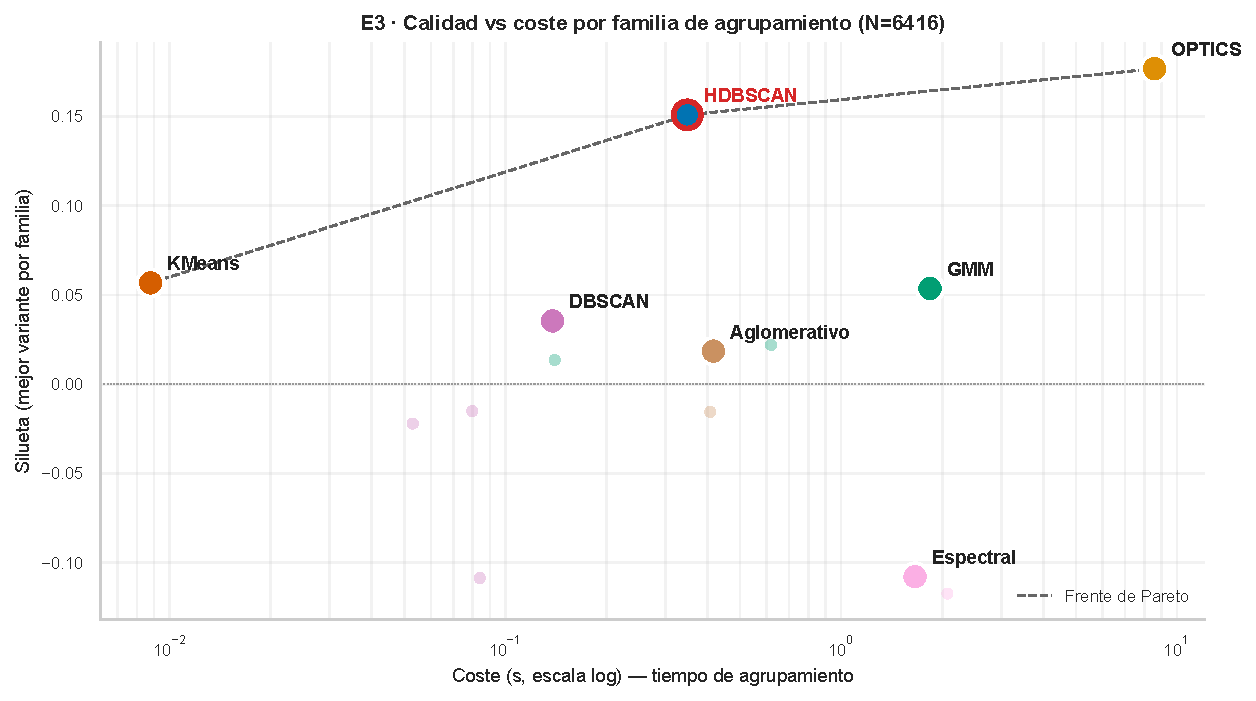
\includegraphics[width=\linewidth]{figures/e3_pareto_quality_cost.pdf}
  \caption[E3, calidad frente a coste por familia]{E3: calidad frente a coste por familia a $N=6416$ (eje horizontal
  logarítmico). La línea discontinua marca el frente de Pareto: HDBSCAN (rojo)
  domina a todas excepto a OPTICS, que paga $\sim$25 veces más coste por
  $\sim$0.02 más de silueta, y K-medias, el más barato pero con una silueta
  0.094 inferior a la de HDBSCAN.}
  \label{fig:e3-pareto}
\end{figure}

\subsubsection{Granularidad de HDBSCAN.}
El barrido E4 calibra \texttt{min\_cluster\_size} (mcs) entre 5 y 200
(tabla~\ref{tab:e4-mcs-6416}). Los valores altos (100, 200), pese a las mejores
métricas intrínsecas, son degenerados: solo producen dos clústeres masivos. El
caso de 50 ($k=4$, coincidente con las cuatro categorías de estilo del extractor)
es algo más defendible. Se escoge \texttt{mcs}=5 como valor base por la
preferencia por un número de clústeres más alto y la sospecha de que
\texttt{mcs}=50 es un agrupamiento demasiado grueso; el experimento E8a refuerza
esta decisión, al favorecer las métricas supervisadas la configuración escogida.

{\footnotesize
\begin{longtable}{|p{1.4cm}|p{1.0cm}|p{1.0cm}|p{1.0cm}|p{1.2cm}|p{1.0cm}|p{1.0cm}|} \hline
  \textbf{mcs} & \textbf{cls} & \textbf{ruido} & \textbf{sil} & \textbf{CH} & \textbf{DB} & \textbf{csCV} \\ \hline
  \endhead
    5 & 563 & 0.199 & 0.151 &   33 & \textbf{1.70} & \textbf{0.75} \\ \hline
   10 & 154 & 0.277 & 0.037 &   56 & 2.20 & 1.78 \\ \hline
   25 &  26 & 0.228 & 0.047 &  209 & 2.66 & 1.81 \\ \hline
   50 &   4 & \textbf{0.026} & \textbf{0.193} & \textbf{1404} & 2.01 & 0.86 \\ \hline
  100 &   2 & 0.008 & 0.269 & 2765 & 1.27 & 0.40 \\ \hline
  200 &   2 & 0.011 & 0.270 & 2776 & 1.27 & 0.40 \\ \hline
  \caption[E4, barrido de \texttt{min\_cluster\_size} a $N=6416$]{E4, barrido de \texttt{min\_cluster\_size} a $N=6416$. La silueta y
  el CH alcanzan su máximo en los valores degenerados ($k{=}2$); el criterio
  conjunto sitúa el óptimo en \texttt{mcs}=5. \glosacalidad}
  \label{tab:e4-mcs-6416}
\end{longtable}
}

\subsubsection{Impacto del segmentador.}
El barrido E5 compara cuatro opciones de segmentación manteniendo fijo el resto
del \textit{pipeline} (tabla~\ref{tab:e5-segmenter-6416}). A escala completa, la
identidad gana en todos los ejes: silueta más alta (0.151), ruido más bajo
(0.199) y mejor coste de ingesta. Los detectores base (YOLO11s/m) recortan
$\sim$1.03 cajas por imagen, reproduciendo el conjunto original con una ganancia
nula o negativa y un sobrecoste del 44\%. El detector \textit{fine-tuned} lidera
a $N=1000$, pero a $N=6416$ obtiene 2.4 recortes por imagen y degenera el
agrupamiento (29.8\% de ruido, 1049 clústeres) con un coste de ingesta 74\%
mayor. Sus métricas de validación lo explican (precisión $0.849$,
\textit{recall} $0.741$, mAP@0.5 $0.808$): produce recortes de calidad variable
que, sumados a que el extractor base no se entrenó con recortes de este tipo,
deterioran la calidad al crecer $N$. La configuración base queda fijada como
\texttt{dinov2\_graffiti\_style\_head}~+~UMAP-10~+~HDBSCAN
\texttt{mcs}=5~+~segmentador identidad~+~SQLite.

{\footnotesize
\begin{longtable}{|p{2.5cm}|p{1.5cm}|p{1.0cm}|p{1.0cm}|p{1.1cm}|p{1.0cm}|p{1.0cm}|p{1.4cm}|} \hline
  \textbf{Segmentador} & \textbf{recortes} & \textbf{r/img} & \textbf{cls} & \textbf{ruido} & \textbf{sil} & \textbf{CH} & \textbf{ingesta (s)} \\ \hline
  \endhead
  identidad           & 6416  & 1.00 &  563 & \textbf{0.199} & \textbf{0.151} & 33.1 & \textbf{1235.5} \\ \hline
  YOLO11s             & 6590  & 1.03 &  502 & 0.225 & 0.127 & 30.4 & 1777.0 \\ \hline
  YOLO11m             & 6603  & 1.03 &  506 & 0.230 & 0.131 & 29.5 & 1811.6 \\ \hline
  YOLO11m \textit{ft} & 15362 & 2.39 & 1049 & 0.298 & 0.122 & \textbf{36.2} & 2152.3 \\ \hline
  \caption[E5, calidad y coste de ingesta a $N=6416$]{E5, calidad intrínseca y coste de ingesta a $N=6416$
  (r/img=recortes por imagen). Cada segmentador alimenta a HDBSCAN un conjunto
  distinto de puntos.}
  \label{tab:e5-segmenter-6416}
\end{longtable}
}

\subsection{Coste computacional}
\label{subsec:res-coste}
Este es uno de los ejes centrales del trabajo: caracterizar empíricamente cómo
crece el coste de cada etapa con $N$ y contrastar las pendientes observadas con
las clases de complejidad teóricas. El rango disponible ($N\le6416$) es estrecho
para separar asintóticamente $O(n\log n)$ de $O(n^2)$, por lo que las pendientes
se reportan como observadas en este régimen y no como exponentes asintóticos.

\subsubsection{Escalabilidad por etapa.}
El barrido E7 mide ingesta, reducción, agrupamiento y búsqueda sobre seis
tamaños; las tablas~\ref{tab:e7-cost} y~\ref{tab:e7-slopes} consolidan los
tiempos por etapa y las pendientes log-log (figura~\ref{fig:e7-scaling}). El
rango reducido de $N$ provoca que varias etapas (DBSCAN, OPTICS) presenten
pendientes inferiores a su complejidad teórica, mientras HDBSCAN y el aglomerativo
exhiben pendientes superiores a 1. El agrupamiento es despreciable a esta escala
(nunca supera los 5~s); el único cuello del agrupamiento es el aglomerativo, que
materializa una matriz $O(n^2)$ de distancias y consume 314~MB a $N=6416$. La
búsqueda SQLite presenta la pendiente esperada ($\approx2.10$): a $N=6416$ una
pasada de 6416 consultas tarda 54.4~minutos, más que la propia ingesta
(21.6~min), y el \textit{throughput} cae de 68 a 2 consultas/s, lo que motiva
directamente el barrido de \textit{backend} (\ref{subsubsec:res-similaritysearch}).
La anomalía más relevante está en UMAP: crece hasta $N=3500$ con pendiente 1.15,
pero a $N=6416$ cae un 47\% porque supera el umbral interno que activa el cálculo
aproximado de vecinos con \texttt{pynndescent}, lo que justifica reportar dos
pendientes distintas.

{\footnotesize
\begin{longtable}{|p{1.0cm}|p{1.6cm}|p{1.2cm}|p{2.0cm}|p{2.0cm}|p{1.4cm}|p{2.0cm}|} \hline
  \textbf{$N$} & \textbf{ingesta (s)} & \textbf{red (s)} & \textbf{HDBSCAN (s)} & \textbf{K-medias (s)} & \textbf{aglo (s)} & \textbf{búsqueda (s)} \\ \hline
  \endhead
   250 &   58.7 &  0.253 & 0.0038 & 0.0025 & 0.0019 &   3.66 \\ \hline
   500 &  115.7 &  0.603 & 0.0069 & 0.0027 & 0.0046 &  16.32 \\ \hline
  1000 &  231.6 &  1.514 & 0.0144 & 0.0033 & 0.0117 &  63.28 \\ \hline
  2000 &  455.9 &  4.542 & 0.1106 & 0.0047 & 0.0427 & 306.81 \\ \hline
  3500 &  776.0 & 11.870 & 0.1863 & 0.0066 & 0.1405 & 995.52 \\ \hline
  6416 & 1294.9 &  6.237 & 0.3580 & 0.0098 & 0.5988 & 3266.60 \\ \hline
  \caption[E7, tiempo por etapa frente a $N$]{E7, tiempo por etapa frente a $N$ (extracto). A $N=6416$ la búsqueda
  SQLite domina absolutamente, con la ingesta como segundo coste.}
  \label{tab:e7-cost}
\end{longtable}
}

{\footnotesize
\begin{longtable}{|p{2.5cm}|p{3.4cm}|p{2.6cm}|p{2.6cm}|} \hline
  \textbf{Etapa / Algoritmo} & \textbf{Escala teórica} & \textbf{Pendiente $N{=}250\ldots6416$} & \textbf{Pendiente $N{=}500\ldots3500$} \\ \hline
  \endhead
  Ingesta (DINOv2)       & $O(n)$            & 0.95 & --   \\ \hline
  Reducción (UMAP)       & $\sim O(n^{1.14})$ & 1.15 & 1.53 \\ \hline
  K-medias ($k$ fijo)      & $\approx O(n)$    & 0.43 & 0.46 \\ \hline
  DBSCAN                 & $O(n\log n)$--$O(n^2)$ & 0.99 & 1.10 \\ \hline
  OPTICS                 & $O(n\log n)$--$O(n^2)$ & 0.94 & 0.98 \\ \hline
  HDBSCAN                & $O(n\log n)$ amort. & 1.53 & 1.84 \\ \hline
  Aglomerativo           & $O(n^2 \log n)$   & 1.77 & 1.76 \\ \hline
  Búsqueda (SQLite)      & $O(n^2)$ por pasada & \textbf{2.10} & 2.13 \\ \hline
  \caption[E7, pendientes observadas por etapa]{E7, pendientes observadas (regresión log-log) por etapa frente a la
  complejidad teórica. La ventana $500\ldots3500$ excluye el punto $N=6416$ de
  reducción (anomalía \texttt{pynndescent}).}
  \label{tab:e7-slopes}
\end{longtable}
}

\begin{figure}[h!]
  \centering
  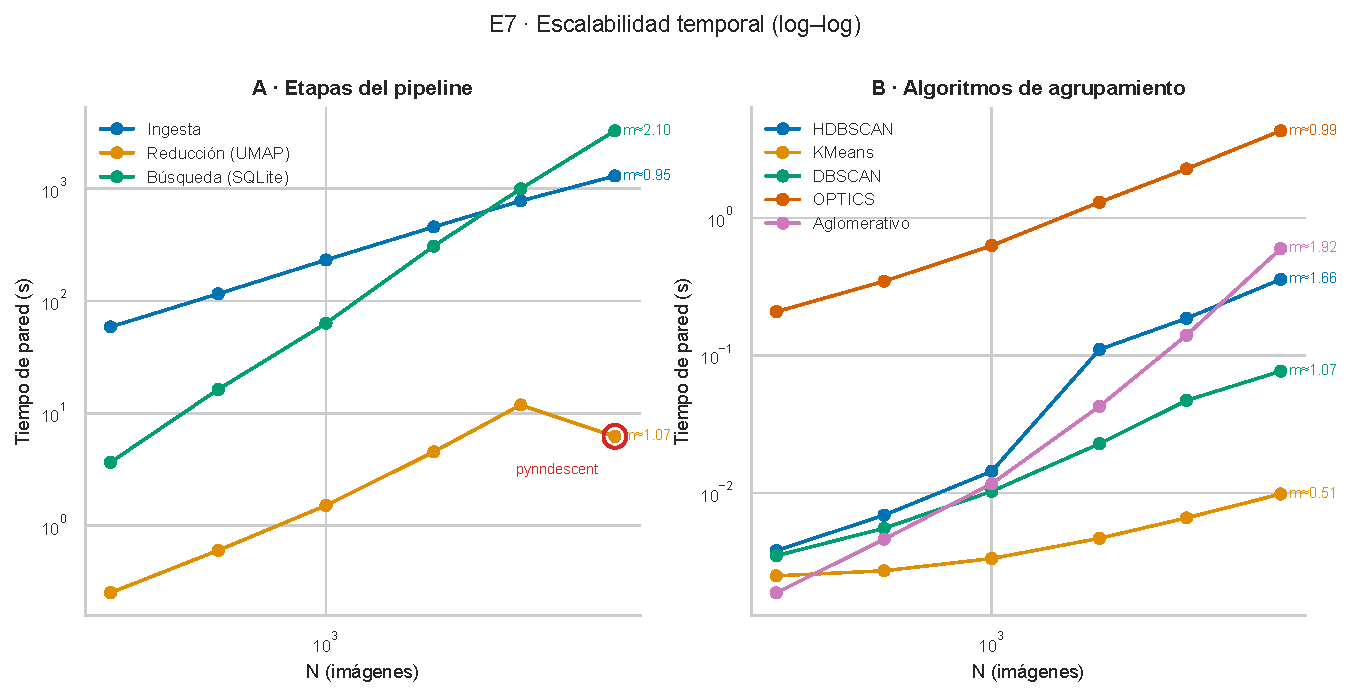
\includegraphics[width=\linewidth]{figures/e7_scalability_loglog.pdf}
  \caption[E7, tiempo de pared vs $N$ por etapa]{E7: tiempo de pared vs $N$ por etapa del \textit{pipeline}, escala
  log-log. La pendiente de la búsqueda SQLite ($\approx2.10$) confirma el coste
  $O(n^2)$ por pasada; la caída de UMAP a $N=6416$ refleja el cambio interno a
  \texttt{pynndescent}.}
  \label{fig:e7-scaling}
\end{figure}

\subsubsection{Búsqueda por similitud: \textit{backend} e índice ANN.}
\label{subsubsec:res-similaritysearch}
El cuello $O(n^2)$ de SQLite motiva el barrido E6 sobre tres \textit{backends}
(tabla~\ref{tab:e6-storage}): SQLite, pgvector exacto y pgvector con HNSW
(\texttt{m}=16, \texttt{ef\_construction}=64). SQLite mantiene un
\textit{throughput} plano ($\sim$150~ips) con tiempo lineal en $N$; pgvector
exacto lo eleva dos órdenes de magnitud, pero por debajo de $N=1000$ está
dominado por el \textit{round-trip} de la conexión. HNSW es el único cuyo
\textit{throughput} crece con $N$: a $N=6416$ es 3.2 veces más rápido que el
exacto y 240 veces más rápido que SQLite, con R@5~=~1.000 a las cuatro escalas, y
su índice se amortiza en una sola consulta frente a SQLite. El barrido
complementario E9 (figura~\ref{fig:similaritysearch-pareto}) recorre once
configuraciones del índice: ninguna baja de \textit{recall} 0.990, y alcanzar
\textit{recall} 1.000 sin penalizar la latencia es posible subiendo \texttt{m} o
\texttt{ef\_construction}, preferibles en un flujo de \enquote{ingesta única,
muchas consultas} porque su sobrecoste se amortiza una vez. HNSW es, por tanto,
la elección por defecto recomendada; SQLite queda como \textit{backend} de
desarrollo de muy pequeña escala.

{\footnotesize
\begin{longtable}{|p{1.0cm}|p{2.6cm}|p{1.6cm}|p{2.0cm}|p{1.6cm}|p{1.8cm}|} \hline
  \textbf{$N$} & \textbf{Backend} & \textbf{ss (s)} & \textbf{ips} & \textbf{idx (s)} & \textbf{R@5} \\ \hline
  \endhead
   500 & SQLite             & 3.05  &    164 & --     & --    \\ \hline
   500 & PostgreSQL exacto  & 0.162 &  3 096 & 0.0    & --    \\ \hline
   500 & PostgreSQL + HNSW  & 0.164 &  3 042 & 0.066  & 1.000 \\ \hline
  1000 & SQLite             & 6.41  &    156 & --     & --    \\ \hline
  1000 & PostgreSQL exacto  & 0.190 &  5 257 & 0.0    & --    \\ \hline
  1000 & PostgreSQL + HNSW  & 0.187 &  5 353 & 0.136  & 1.000 \\ \hline
  2500 & SQLite             & 16.89 &    148 & --     & --    \\ \hline
  2500 & PostgreSQL exacto  & 0.234 & 10 678 & 0.0    & --    \\ \hline
  2500 & PostgreSQL + HNSW  & 0.166 & 15 092 & 0.372  & 1.000 \\ \hline
  6416 & SQLite             & 43.10 &    149 & --     & --    \\ \hline
  6416 & PostgreSQL exacto  & 0.578 & 11 109 & 0.0    & --    \\ \hline
  6416 & PostgreSQL + HNSW  & 0.179 & 35 936 & 0.465  & 1.000 \\ \hline
  \caption[E6, latencia y \textit{recall} por \textit{backend}]{E6, latencia, \textit{throughput} y \textit{recall} por
  \textit{backend} y tamaño de banco. HNSW solo se separa visiblemente por encima
  de $N\approx2500$; el dataset del trabajo está por encima de ese cruce.}
  \label{tab:e6-storage}
\end{longtable}
}

\begin{figure}[h!]
  \centering
  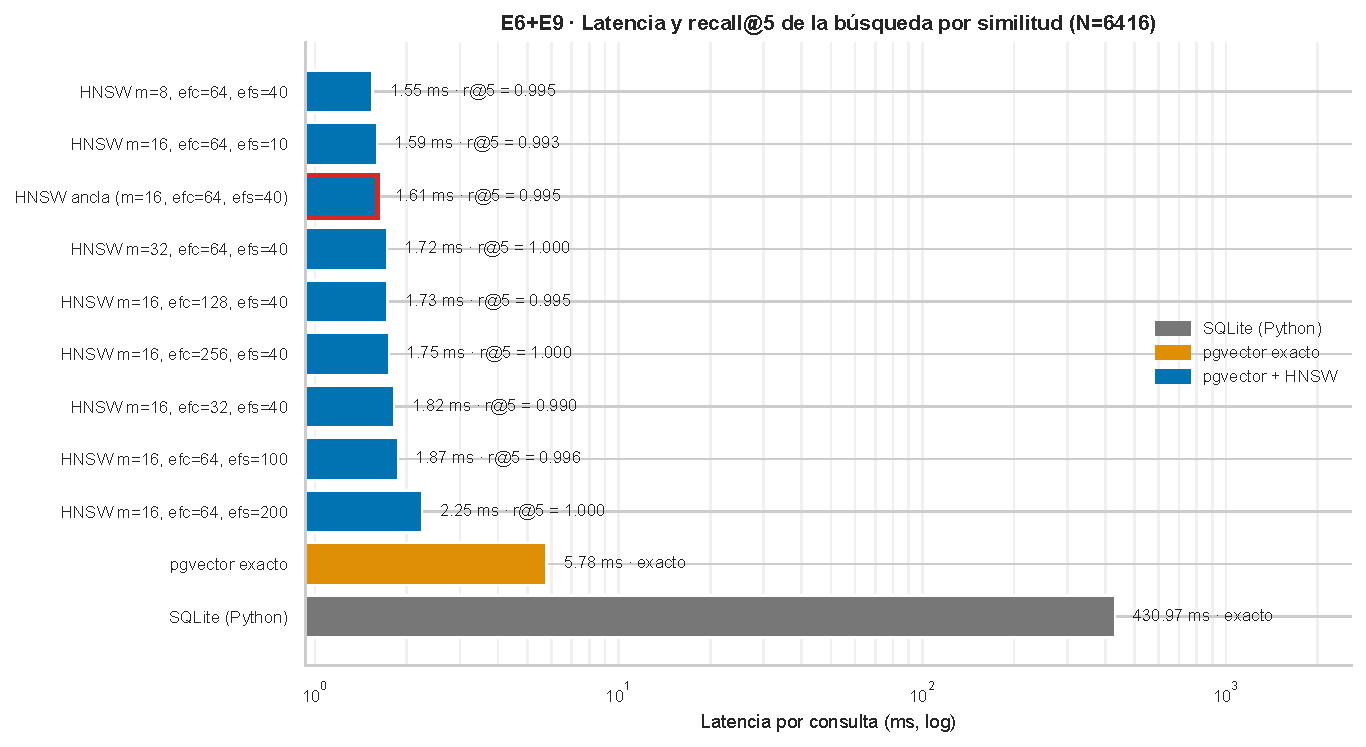
\includegraphics[width=\linewidth]{figures/e6_e9_pareto.pdf}
  \caption[E6+E9, latencia y \texttt{R@5} por configuración HNSW]{E6+E9: latencia por consulta (eje logarítmico) y \textit{recall}@5
      por \textit{backend} y configuración HNSW a $N=6416$. La configuración del
      barrido E6 aparece en rojo; SQLite y pgvector exacto se incluyen como
      referencia.}
  \label{fig:similaritysearch-pareto}
\end{figure}

\subsection{Validación supervisada}
\label{subsec:res-supervisada}
Las métricas extrínsecas miden directamente la concordancia entre los clústeres y
la verdad de referencia sobre los dos conjuntos etiquetados por estilo y autoría
(unidad de análisis: el recorte, segmentador identidad; 294 recortes sobre 4
estilos para E8a, 185 sobre 87 autores para E8b). Los dos diseños no son
simétricos en su exposición al cambio de dominio: la cabeza estilística se
entrenó sobre un conjunto mixto y se evalúa sobre Salamanca disjunto (un
\textit{held-out} dentro del dominio de entrenamiento), mientras que las de
autoría se entrenaron solo con Cuenca, así que E8b mezcla generalización a
autores no vistos con un desplazamiento Cuenca$\to$Salamanca.

\subsubsection{Evaluación por estilo.}
La tabla~\ref{tab:e8a-best} recoge la mejor celda por extractor, seleccionada por
el ARI por defecto. El resultado es inequívoco: la cabeza estilística de DINOv2 +
identidad + K-medias-4 obtiene ARI~=~0.722 y F1~=~0.806, más del doble del ARI de
cualquier otro extractor sin entrenar, seguida por la cabeza de MobileNetV3
(0.627). Las cabezas de \emph{autoría} no solo no mejoran el ARI de estilo
respecto a su \textit{backbone}, sino que lo empeoran (DINOv2 $0.356\to0.302$):
el \textit{fine-tuning} concentra el eje para el que fue entrenado y deja al otro
en desventaja, una matriz de transferencia diagonal-dominante que evidencia que
las dos cabezas codifican información distinta. La señal de recuperación
supervisada ($k=5$) confirma el ordenamiento sin depender del agrupador: la cabeza
estilística de DINOv2 lidera los tres índices (P@5~=~0.851, MAP@5~=~0.909,
MRR~=~0.922), lo que descarta que su liderazgo esté inducido por la elección de
agrupador.

{\footnotesize
\begin{longtable}{|p{5.0cm}|p{1.1cm}|p{1.0cm}|p{1.0cm}|p{1.0cm}|p{2.9cm}|} \hline
  \textbf{Extractor} & \textbf{ARI} & \textbf{NMI} & \textbf{F1} & \textbf{sil} & \textbf{Celda} \\ \hline
  \endhead
  \texttt{dinov2\_graffiti\_style\_head}      & \textbf{0.722} & \textbf{0.678} & \textbf{0.806} & \textbf{0.284} & ident.\ + K-medias-4   \\ \hline
  \texttt{mob.\_graffiti\_style\_head}        & 0.627 & 0.539 & 0.740 & 0.272 & ident.\ + K-medias-4   \\ \hline
  \texttt{clip\_vit\_b32}                     & 0.368 & 0.392 & 0.556 & 0.047 & UMAP + aglomerativo    \\ \hline
  \texttt{dinov2\_vits14}                     & 0.356 & 0.374 & 0.558 & 0.135 & ident.\ + K-medias-4   \\ \hline
  \texttt{mobilenet\_v3}                      & 0.356 & 0.336 & 0.550 & 0.038 & UMAP + aglomerativo    \\ \hline
  \texttt{resnet50}                           & 0.334 & 0.277 & 0.548 & 0.058 & ident.\ + espectral  \\ \hline
  \texttt{mob.\_graffiti\_author\_head}       & 0.318 & 0.295 & 0.517 & 0.046 & UMAP + aglomerativo    \\ \hline
  \texttt{dinov2\_graffiti\_author\_head}     & 0.302 & 0.273 & 0.519 & 0.094 & UMAP + aglomerativo    \\ \hline
  \caption[E8a, mejor celda por extractor (estilo)]{E8a, mejor celda por extractor sobre la evaluación de estilo (294
  recortes, 4 clases). Las cabezas de autoría quedan por debajo del
  \textit{backbone} en ambas familias.}
  \label{tab:e8a-best}
\end{longtable}
}

Una revisión manual revela que HDBSCAN no distingue las cuatro categorías como
clústeres separados, sino que las agrupa en tres conjuntos
(figura~\ref{fig:e8a-hdbscan}): \enquote{sencillos} ($\sim$150 recortes,
mayoritariamente \textit{tags}), \enquote{elaborados} ($\sim$120 recortes,
\textit{throw-ups} elaborados y \textit{pieces}) y \enquote{characters} (17
recortes).

\begin{figure}[h!]
  \centering
  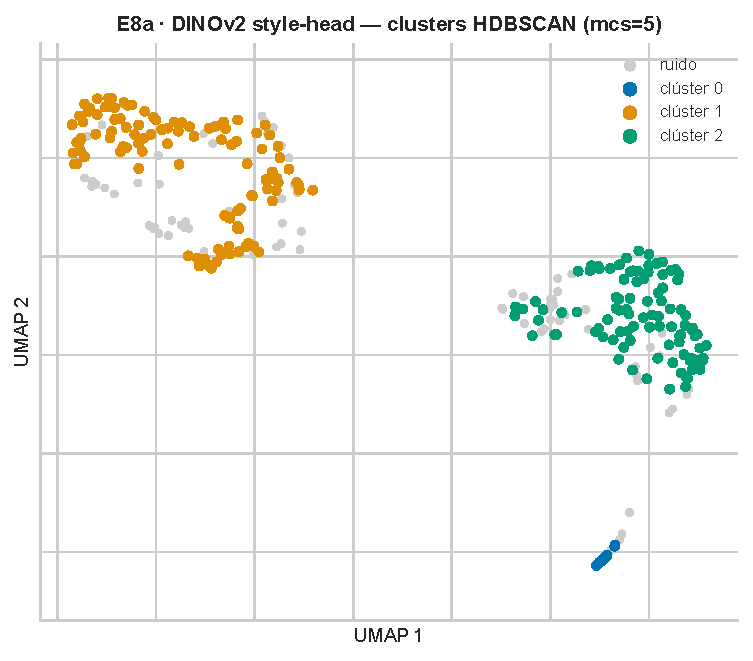
\includegraphics[width=0.85\linewidth]{figures/e8a_hdbscan_3clusters.pdf}
  \caption[Distribución 2D de los recortes de E8a por clúster HDBSCAN]{Representación bidimensional de los recortes de E8a en el espacio de la
    cabeza estilística de DINOv2, coloreados por los tres clústeres de HDBSCAN.}
  \label{fig:e8a-hdbscan}
\end{figure}

\subsubsection{Evaluación por autor.}
E8b parte de una hipótesis simétrica a E8a, pero la tabla~\ref{tab:e8b-best}
muestra que no se cumple: el mejor ARI lo obtiene CLIP (0.076) y los ocho
extractores caben en una banda 0.041--0.076 cercana al azar (la celda ganadora de
E8a vale 0.722, $\sim$10 veces más). Es un resultado negativo pero esperado: la
clasificación por estilo es mucho más sencilla que el agrupamiento por autoría,
agravado por un cambio de dominio severo y un conjunto de peor calidad. No
invalida las cabezas de autoría, sino que indica que el conjunto anotado es
insuficiente; serían necesarios muchos más recortes y autores, o un
pre-entrenamiento no supervisado previo al \textit{fine-tuning}. La recuperación
sigue la misma tendencia, con las cabezas de autoría por debajo de los
extractores sin entrenar.

{\footnotesize
\begin{longtable}{|p{5.0cm}|p{1.1cm}|p{1.0cm}|p{1.0cm}|p{1.0cm}|p{2.9cm}|} \hline
  \textbf{Extractor} & \textbf{ARI} & \textbf{NMI} & \textbf{F1} & \textbf{sil} & \textbf{Celda} \\ \hline
  \endhead
  \texttt{clip\_vit\_b32}                     & \textbf{0.076} & \textbf{0.789} & 0.090 & 0.003 & UMAP + aglo-87 \\ \hline
  \texttt{dinov2\_graffiti\_author\_head}     & 0.065 & 0.647 & \textbf{0.093} & 0.052 & UMAP + aglo-30 \\ \hline
  \texttt{dinov2\_vits14}                     & 0.055 & 0.754 & 0.079 & \textbf{0.096} & ident.\ + aglo-87 \\ \hline
  \texttt{dinov2\_graffiti\_style\_head}      & 0.054 & 0.628 & 0.085 & 0.037 & UMAP + aglo-30 \\ \hline
  \texttt{resnet50}                           & 0.049 & 0.778 & 0.064 & 0.028 & UMAP + aglo-87 \\ \hline
  \texttt{mob.\_graffiti\_author\_head}       & 0.048 & 0.627 & 0.077 & 0.021 & UMAP + aglo-30 \\ \hline
  \texttt{mobilenet\_v3}                      & 0.046 & 0.780 & 0.060 & 0.023 & UMAP + aglo-87 \\ \hline
  \texttt{mob.\_graffiti\_style\_head}        & 0.041 & 0.629 & 0.070 & 0.020 & UMAP + aglo-30 \\ \hline
  \caption[E8b, mejor celda por extractor (autoría)]{E8b, mejor celda por extractor sobre la evaluación de autoría
  (185 recortes, 87 autores, Cuenca$\to$Salamanca). Todos los ARI caen en una
  banda estrecha cercana al suelo.}
  \label{tab:e8b-best}
\end{longtable}
}

\subsubsection{Correlación interna-externa.}
Sobre E8a y E8b se calcula la correlación de Pearson entre la silueta y el ARI a
nivel de celda. En E8a (4 clases) es positiva y significativa ($r=+0.78$, $n=48$,
$p<10^{-7}$ sobre los agrupadores de $k$ fijo; $r=+0.55$ al incluir HDBSCAN). En
E8b (87 clases) el signo se invierte ($r=-0.54$), pero sin peso práctico, ya que
todo el rango de ARI vive cerca del azar: no indica que la silueta descarte una
estructura de autoría recuperable, sino que tal estructura no existe a este
nivel. El factor común es la granularidad de la verdad de referencia: la silueta
recompensa pocos clústeres grandes y cohesivos, lo que coincide con el ARI a
grano grueso (estilo) pero se opone a grano fino (autoría, donde el mayor ARI
exige $k=87$ clústeres diminutos de silueta casi nula). La consecuencia práctica
es la elección del extractor base: la cabeza estilística de DINOv2, de las peores
por métricas intrínsecas en E1, se escoge por su liderazgo en E8a; haber elegido
por el ranking intrínseco a $N=6416$ habría llevado a una configuración de peor
rendimiento en la tarea que motiva el trabajo.
